
\section{Single planet retrieval}
\label{sec:exp_singles}

Similar to the experiment of retrieving monotransits from LCSim light curves, we now evaluate several methods on their ability of retrieving repeating signals from light curves. To do so, 5000 LCSim light curves were generated, each of 27.4 days and without missing data. 50\% of the light curves were injected with at least three transit signals from a single planet, and 50\% was left without signals. The task was to retrieve the correct epoch $t_0$ and period $P$ of the transit signal. $t_0$ was correct if it is anywhere within the duration of the first transit signal, and $P$ if it was off by no more than 1\% of the correct period.

Again, we used BLS as baseline for this task, which in this case is the standard algorithm that takes into account periodicities. We used \texttt{astropy}'s implementation of BLS\footnote{\url{https://docs.astropy.org/en/stable/timeseries/bls.htmls}}, with build-in heuristics for the trial periods that are searched over. The trial durations of the fitted box function range from 1 to 13 hours with steps of 30 minutes. Prior to applying BLS, the input light curves were detrended with a time-windowed median filter. Window sizes of 6, 12 and 24 hours were used, which are referred to with BLS-6h, BLS-12h and BLS-24h respectively.

We evaluate both PTS-Peak and PTS-Fold in this task, and set the peak threshold for PTS-Peak to 0.25. For each of the methods, the search is limited to signals with at least three repetitions and a minimum period of 2 days, because this was the minimum period used in the simulations. Moreover, each method was only allowed to return a maximum of three candidate detections per input light curve, each accompanied by a value that was used to set a detection threshold. 

Figure \ref{fig:singles-pr} shows the precision-recall curves for each method in the given task. The curves drop down steeper than those in Figure \ref{fig:monos-pr}, which is likely because in this case periodicities are taken into account, which reduce the chance of false detections. In this case however, BLS performed better than the RNN-based detection methods. This was for each of the chosen window sizes for detrending, although a window of 12 hours showed the best results, which is in line with the results of \cite{hippke2019wotan}. Lastly, the PTS-Fold algorithm performed better than PTS-Peak, as expected from Section \ref{sec:exp_algorithm}.


\begin{figure}
    \centering
    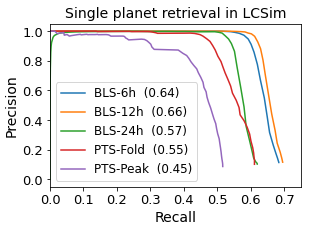
\includegraphics[width=0.4\linewidth]{Experiments/Figures/Singles/singles_PR.png}
    \caption{\todo{caption; between brackets shows area under the curve (AUC), also interpreted as average precision} \todo{explain that we have no uncertainties, and these results therefore only tell something about this specific experiment. future research should confirm these findings.}}
    \label{fig:singles-pr}
\end{figure}